\section{API}
\subsection{Senza autenticazione}
\subsubsection{Login}
\textbf{Tipologia:} POST \\
\textbf{API:} /api/login \\
\textbf{Descrizione:} Necessita di una richiesta con body contenente email e password dell'utente. \\
\textbf{Scenario:} 
\begin{figure}[h]
\centering
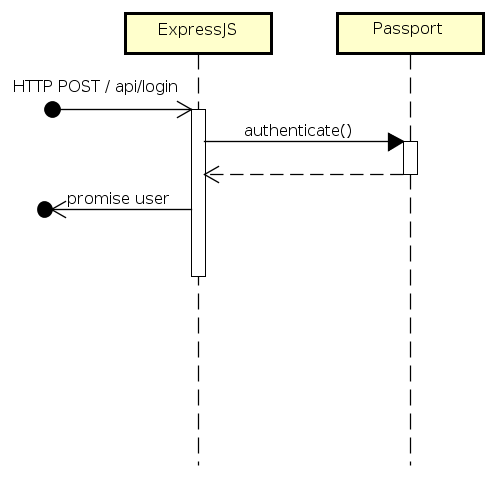
\includegraphics[width=0.8\textwidth]{res/sections/backend/(POST)login.png}
\caption{Scenario del login}
\end{figure}

\newpage
\subsubsection{Registrazione}
\textbf{Tipologia:} POST \\
\textbf{API:} /api/register/:unique\_code \\
\textbf{Descrizione:} Metodo per la creazione di un utente invitato da una company. Necessita di una richiesta con body contenete le informazioni per la creazione completa di un utente \\
\textbf{Scenario:} 
\begin{figure}[h]
\centering
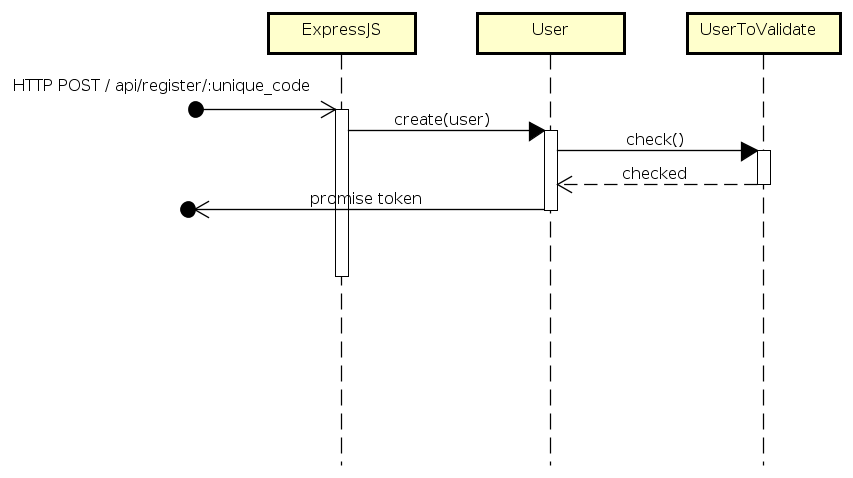
\includegraphics[width=0.8\textwidth]{res/sections/backend/(POST)register.png}
\caption{Scenario della registrazione}
\end{figure}

\newpage
\subsubsection{Creazione Company}
\textbf{Tipologia:} POST \\
\textbf{API:} /api/company \\
\textbf{Descrizione:} Necessita di una richiesta con body contenente le informazioni relative alla company e alla creazione del profilo del suo Owner. \\
\textbf{Scenario:} 
\begin{figure}[h]
\centering
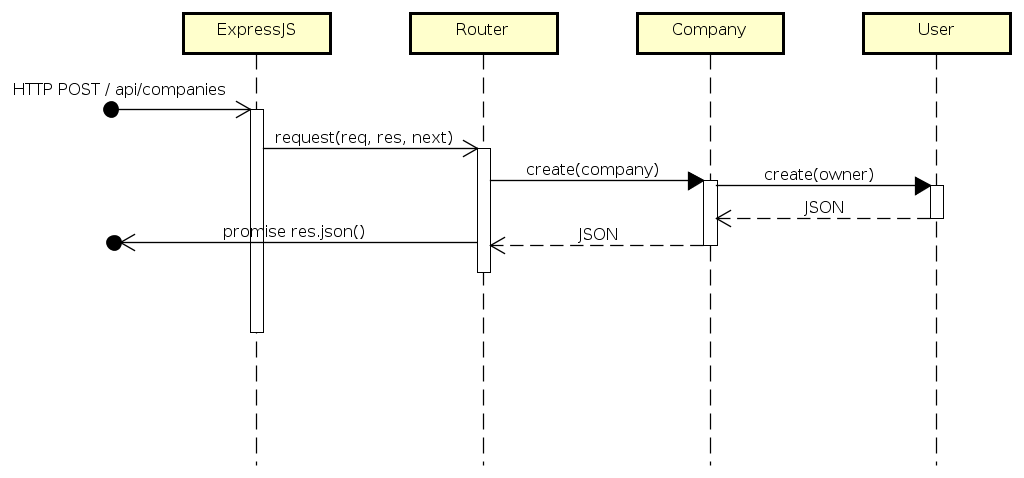
\includegraphics[width=0.8\textwidth]{res/sections/backend/(POST)company.png}
\caption{Scenario della creazione company}
\end{figure}

\newpage
\subsection{User}
\subsubsection{Utenti di una company}
\textbf{Tipologia:} GET \\
\textbf{API:} /api/:company\_id/user \\
\textbf{Livello di accesso minimo:} MEMBER \\
\textbf{Descrizione:} Ritorna un array di JSON contenenti i profili degli utenti della company. \\
\textbf{Scenario:} 
\begin{figure}[h]
\centering
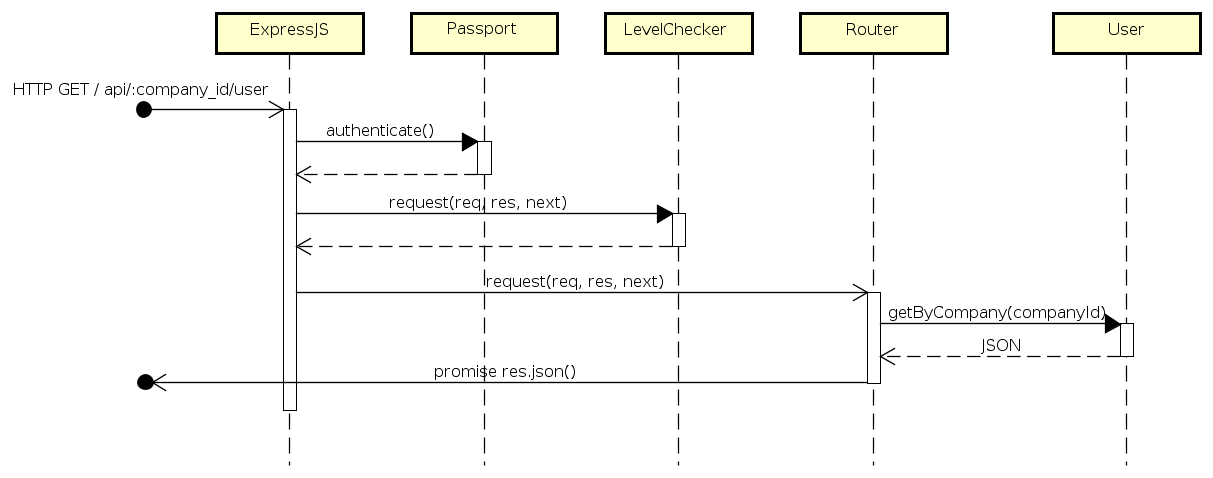
\includegraphics[width=0.8\textwidth]{res/sections/backend/(GET)user.png}
\caption{Scenario della ricerca utenti di una company specifica}
\end{figure}

\newpage
\subsubsection{Inserimento utente}
\textbf{Tipologia:} POST \\
\textbf{API:} /api/:company\_id/user \\
\textbf{Livello di accesso minimo:} ADMIN \\
\textbf{Descrizione:} Necessita di una richiesta con body contenente l'email e il livello di accesso dell'utente.\\
\textbf{Scenario:} 
\begin{figure}[h]
\centering
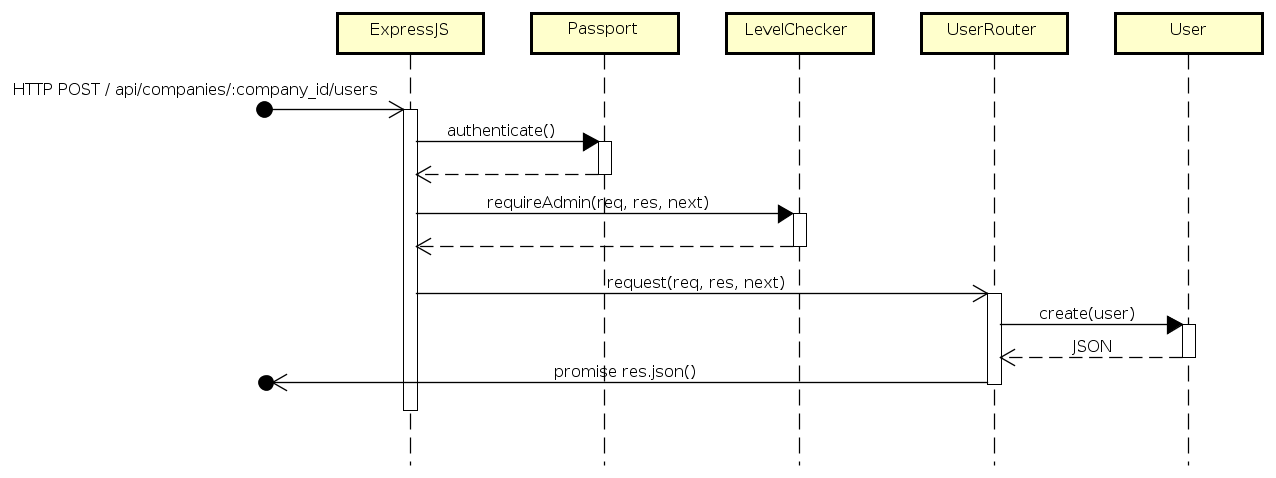
\includegraphics[width=0.8\textwidth]{res/sections/backend/(POST)user.png}
\caption{Scenario dell'inserimento utente in una company}
\end{figure}

\newpage
\subsubsection{Ottenimento del profilo utente}
\textbf{Tipologia:} GET \\
\textbf{API:} /api/:company\_id/user/:user\_id \\
\textbf{Livello di accesso minimo:} GUEST \\
\textbf{Descrizione:} Ritorna un oggetto JSON contenente le informazioni relative al profilo dell'utente indicato da user\_id \\
\textbf{Scenario:} 
\begin{figure}[h]
\centering
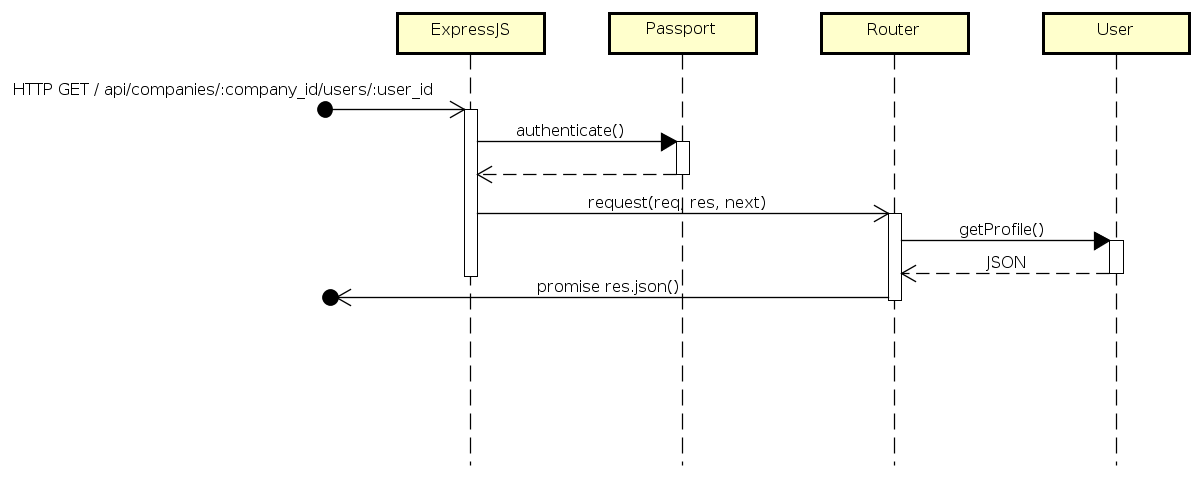
\includegraphics[width=0.8\textwidth]{res/sections/backend/(GET)profiloUtente.png}
\caption{Scenario dell'ottenimento del profilo utente}
\end{figure}

\newpage
\subsubsection{Aggiornamento del profilo utente}
\textbf{Tipologia:} PUT \\
\textbf{API:} /api/:company\_id/user/:user\_id \\
\textbf{Livello di accesso minimo:} GUEST \\
\textbf{Descrizione:} Necessita di una richiesta con un body contenente le informazioni per modificare l'utente indicato da user\_id. Il metodo deve essere utilizzato per la modifica del profilo di un utente. Un utente con permessi inferiori ad ADMIN ha la possibilità di modificare solo i propri dati, mentre ad ADMIN e OWNER vengono permesse modifiche a tutti i profili della company. 
\textbf{Scenario:} 
\begin{figure}[h]
\centering
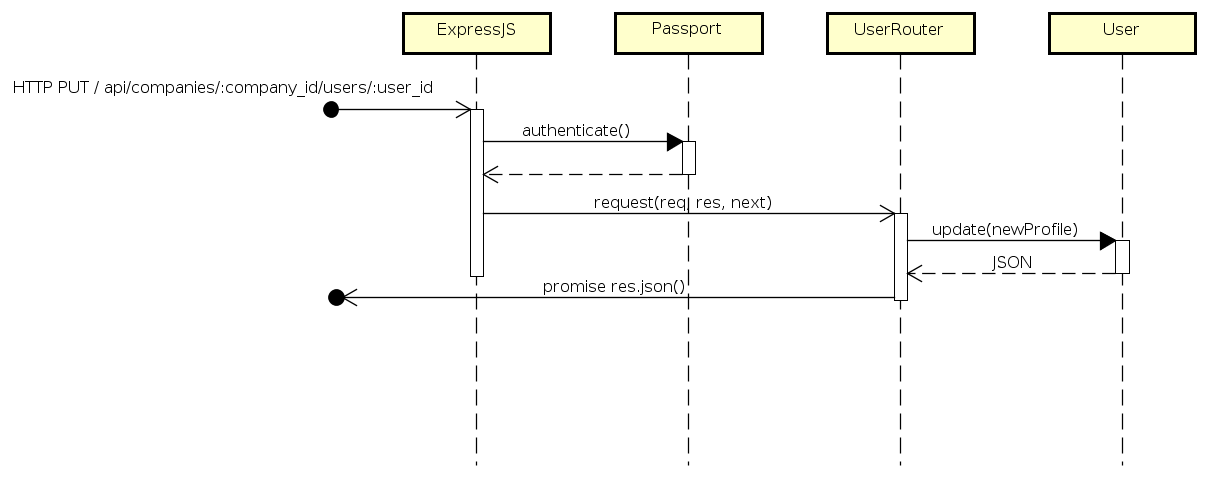
\includegraphics[width=0.8\textwidth]{res/sections/backend/(PUT)profiloUtente.png}
\caption{Scenario dell'aggiornamento del profilo utente}
\end{figure}

\newpage
\subsubsection{Aggiornamento delle credenziali utente}
\textbf{Tipologia:} PUT \\
\textbf{API:} /api/:company\_id/user/:user\_id/credentials \\
\textbf{Livello di accesso minimo:} GUEST \\
\textbf{Descrizione:} Metodo per la modifica delle credenziali di accesso di un utente. Un utente ha il permesso di cambiare solo le proprie credenziali. \\
\textbf{Scenario:} 
\begin{figure}[h]
\centering
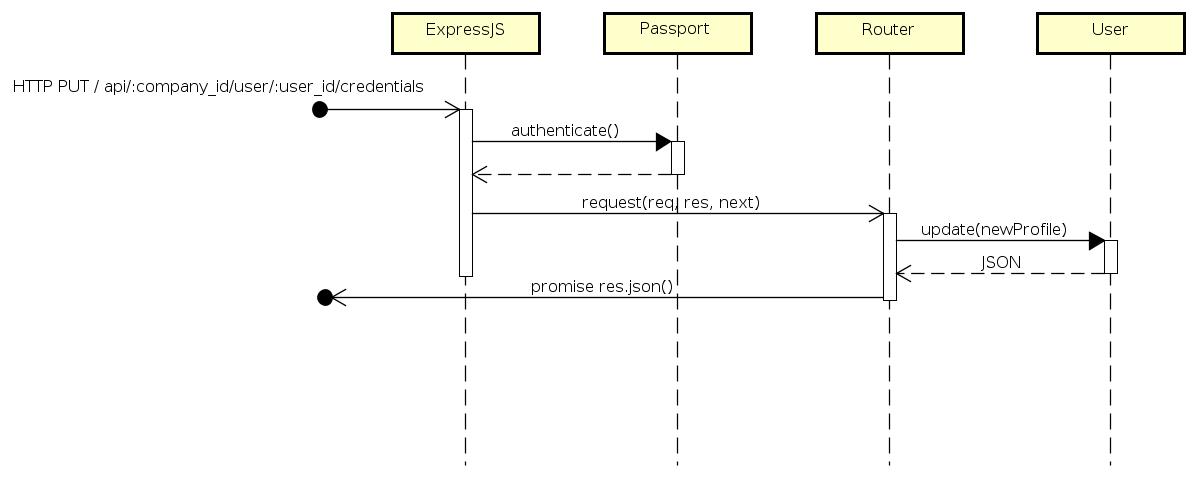
\includegraphics[width=0.8\textwidth]{res/sections/backend/(PUT)credenzialiUtente.png}
\caption{Scenario dell'aggiornamento delle credenziali di un utente}
\end{figure}

\newpage
\subsubsection{Cancellazione utente}
\textbf{Tipologia:} DELETE \\
\textbf{API:} /api/:company\_id/user/:user\_id \\
\textbf{Livello di accesso minimo:} ADMIN \\
\textbf{Descrizione:} Ritorna un messaggio di conferma dell'avvenuta cancellazione. \\
\textbf{Scenario:} 
\begin{figure}[h]
\centering
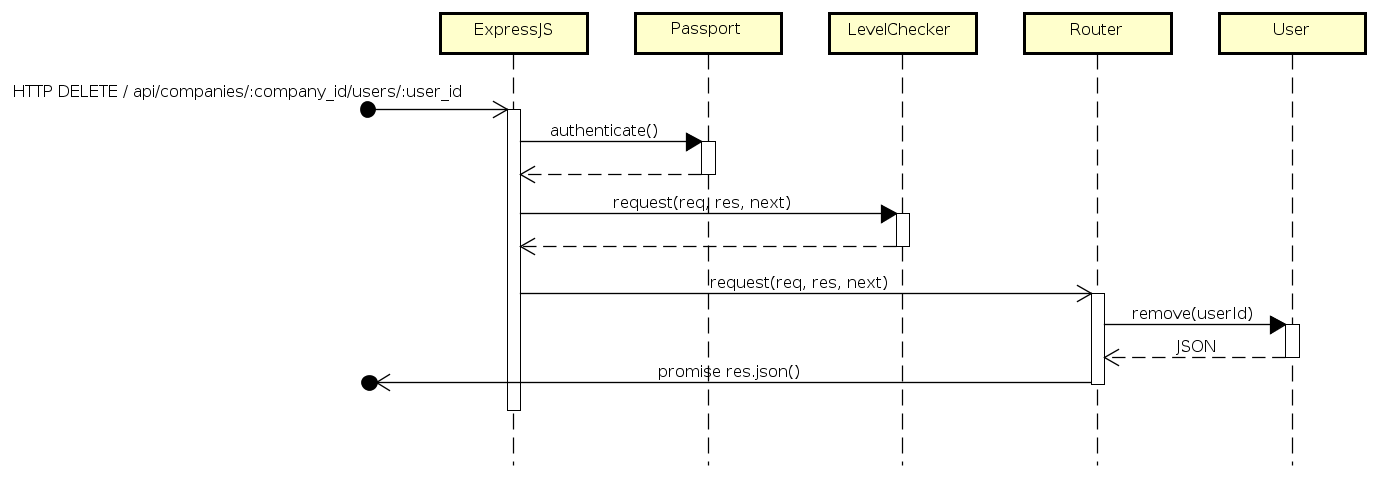
\includegraphics[width=0.8\textwidth]{res/sections/backend/(DELETE)user.png}
\caption{Scenario della cancellazione utente da una company}
\end{figure}

\newpage
\subsection{Company}
\textbf{Tipologia:} GET \\
\textbf{API:} /api/:company\_id/ \\
\textbf{Livello di accesso minimo:} GUEST \\
\textbf{Descrizione:} Ritorna le informazioni generali di una company \\
\textbf{Scenario:} 
\subsubsection{Dati di una company}
\begin{figure}[h]
\centering
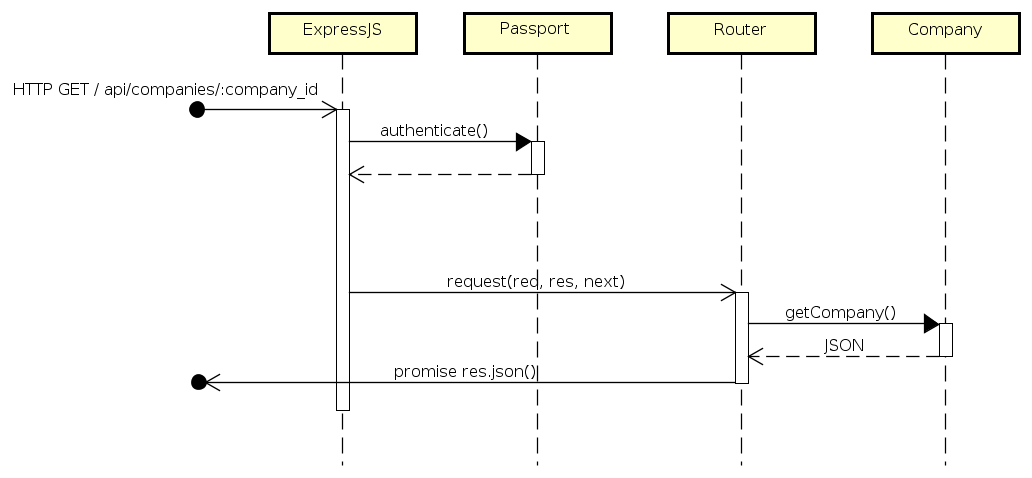
\includegraphics[width=0.8\textwidth]{res/sections/backend/(GET)company.png}
\caption{Scenario di ottenimento dei dati di una company}
\end{figure}

\newpage
\subsubsection{Aggiornamento dei dati di una company}
\textbf{Tipologia:} PUT \\
\textbf{API:} /api/:company\_id/ \\
\textbf{Livello di accesso minimo:} ADMIN \\
\textbf{Descrizione:} Necessita di una richiesta con body contenente le modifiche da apportare ai dati della company. \\
\textbf{Scenario:} 
\begin{figure}[h]
\centering
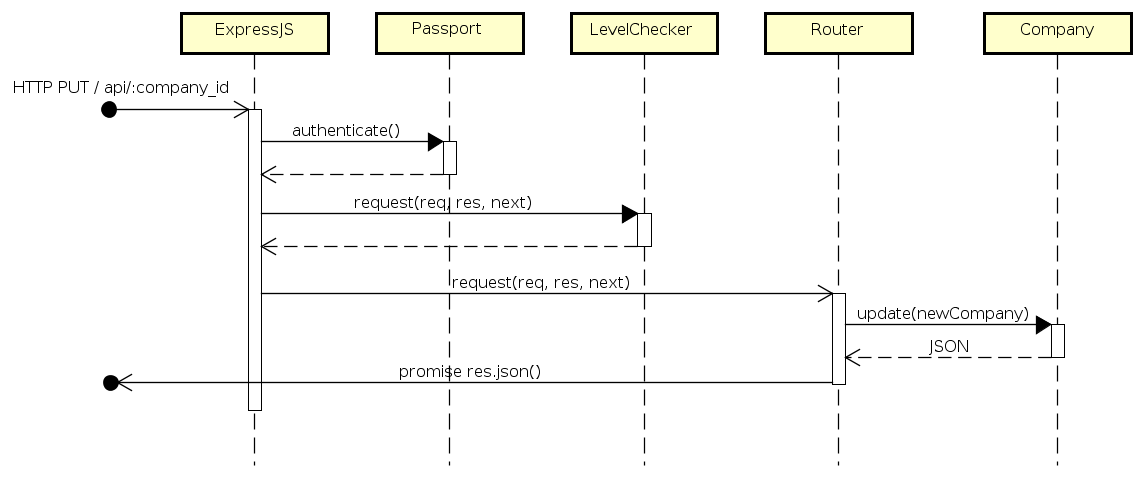
\includegraphics[width=0.8\textwidth]{res/sections/backend/(PUT)company.png}
\caption{Scenario dell'aggiornamento dei dati di una company}
\end{figure}

\newpage
\subsubsection{Cancellazione di una company}
\textbf{Tipologia:} DELETE \\
\textbf{API:} /api/:company\_id/ \\
\textbf{Livello di accesso minimo:} ADMIN \\
\textbf{Descrizione:} Ritorna un messaggio di avvenuta cancellazione. \\
\textbf{Scenario:} 
\begin{figure}[h]
\centering
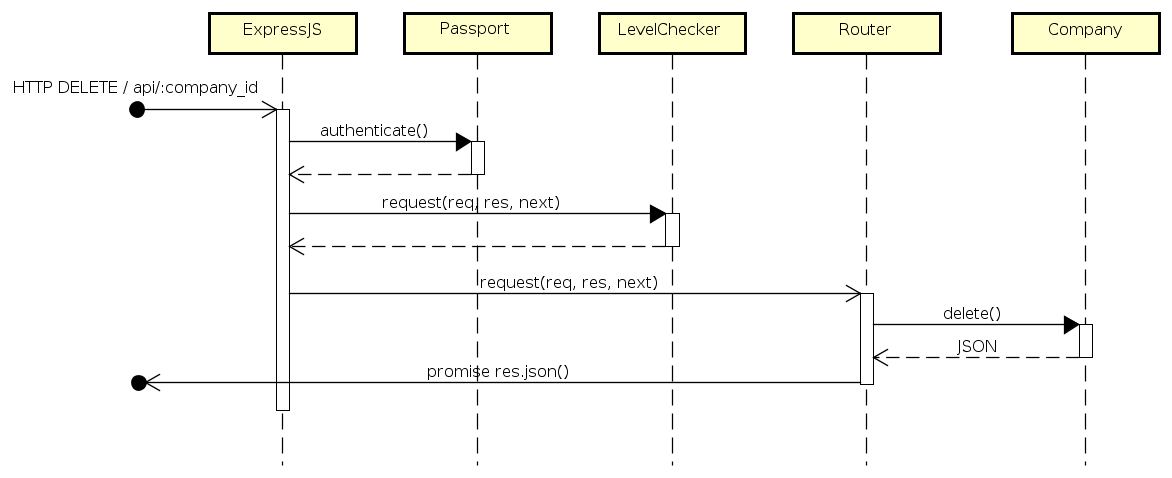
\includegraphics[width=0.8\textwidth]{res/sections/backend/(DELETE)company.png}
\caption{Scenario della cancellazione di una company}
\end{figure}

\newpage
\subsection{DSL}
\subsubsection{Elenco delle specifiche DSL}
\textbf{Tipologia:} GET \\
\textbf{API:} /api/:company\_id/DSL \\
\textbf{Livello di accesso minimo:} GUEST \\
\textbf{Descrizione:} Ritorna un array contenente le DSL in formato JSON. \\
\textbf{Scenario:} 
\begin{figure}[h]
\centering
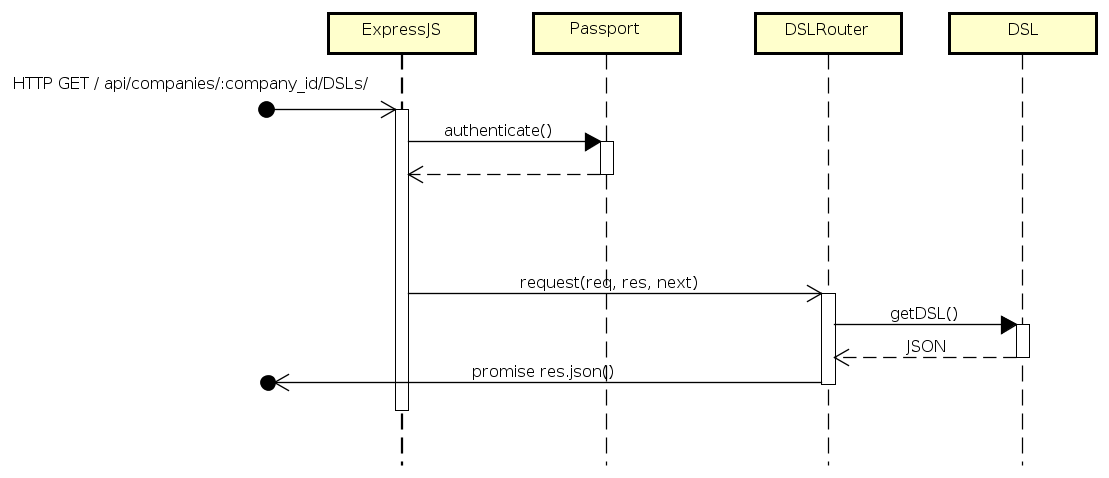
\includegraphics[width=0.8\textwidth]{res/sections/backend/(GET)dsl.png}
\caption{Scenario dell'elenco delle specifiche DSL}
\end{figure}

\newpage
\subsubsection{Lettura del codice di una specifica DSL}
\textbf{Tipologia:} GET \\
\textbf{API:} /api/:company\_id/DSL/:dsl\_id \\
\textbf{Livello di accesso minimo:} GUEST \\
\textbf{Descrizione:} Ritorna la specifica DSL richiesta in formato JSON. \\
\textbf{Scenario:} 
\begin{figure}[h]
\centering
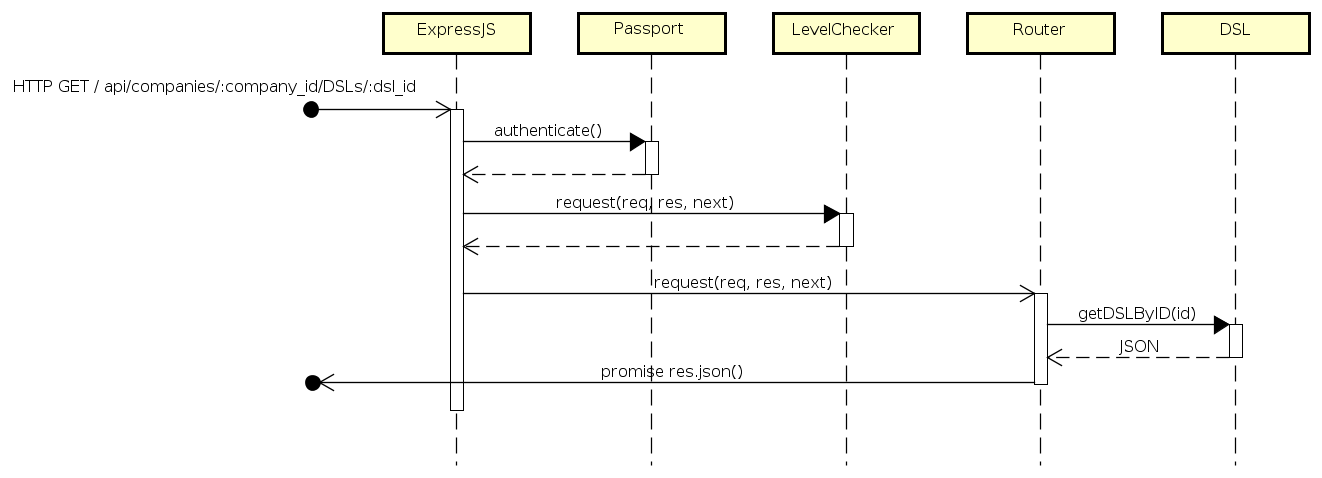
\includegraphics[width=0.8\textwidth]{res/sections/backend/(GET)dslByID.png}
\caption{Scenario della lettura del codice di una specifica DSL}
\end{figure}

\newpage
\subsubsection{Aggiunta di una specifica DSL}
\textbf{Tipologia:} POST \\
\textbf{API:} /api/:company\_id/DSL \\
\textbf{Livello di accesso minimo:} MEMBER \\
\textbf{Descrizione:} Necessita di una richiesta con body contenente i dati necessari alla creazione della DSL. \\
\textbf{Scenario:} 
\begin{figure}[h]
\centering
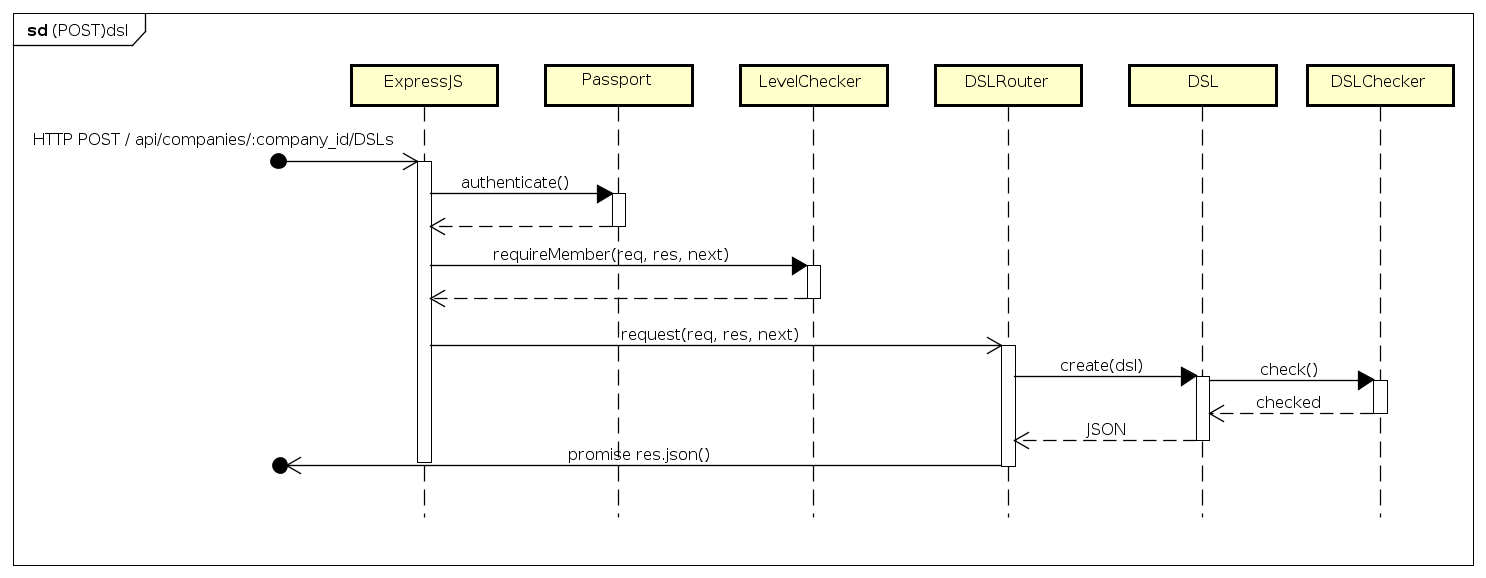
\includegraphics[width=0.8\textwidth]{res/sections/backend/(POST)dsl.png}
\caption{Scenario della creazione di una specifica DSL}
\end{figure}

\newpage
\subsubsection{Aggiornamento del codice di una specifica DSL}
\textbf{Tipologia:} PUT \\
\textbf{API:} /api/:company\_id/DSL/:dsl\_id \\
\textbf{Livello di accesso minimo:} MEMBER \\
\textbf{Descrizione:} Necessita di una richiesta con body contenente i dati necessari alla modifica della DSL specificata da dsl\_id. \\
\textbf{Scenario:}
\begin{figure}[h]
\centering
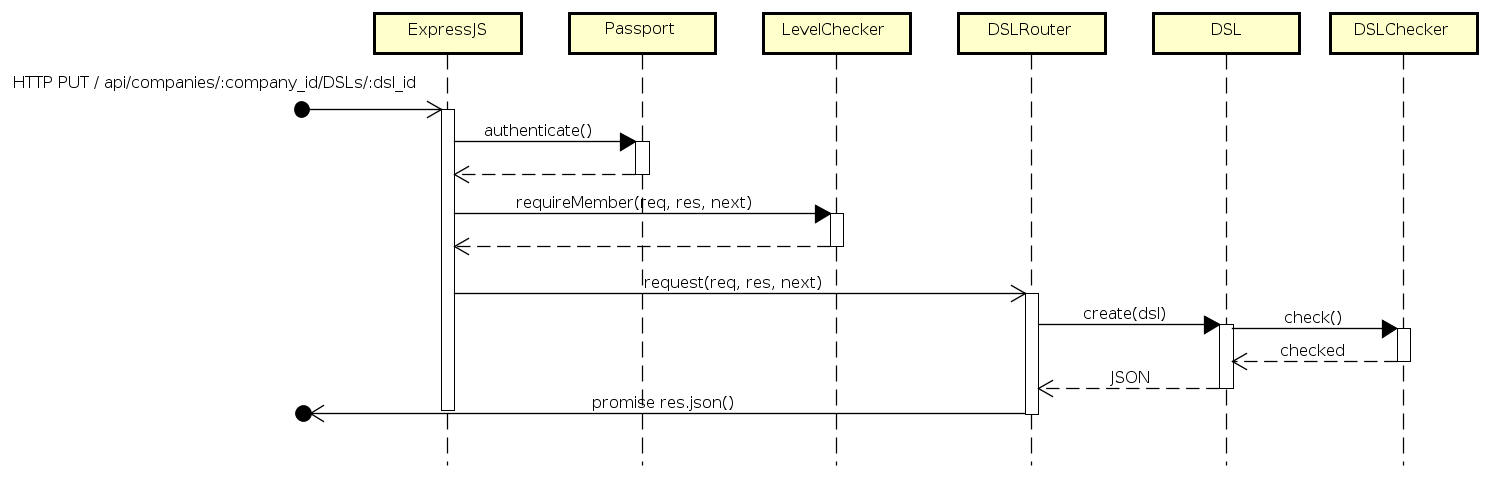
\includegraphics[width=0.8\textwidth]{res/sections/backend/(PUT)dsl.png}
\caption{Scenario dell'aggiornamento del codice di una specifica DSL}
\end{figure}

\newpage
\subsubsection{Cancellazione di una specifica DSL}
\textbf{Tipologia:} DELETE \\
\textbf{API:} /api/:company\_id/DSL/:dsl\_id \\
\textbf{Livello di accesso minimo:} MEMBER \\
\textbf{Descrizione:} Ritorna un messaggio in formato JSON di avvenuta cancellazione. \\
\textbf{Scenario:} 
\begin{figure}[h]
\centering
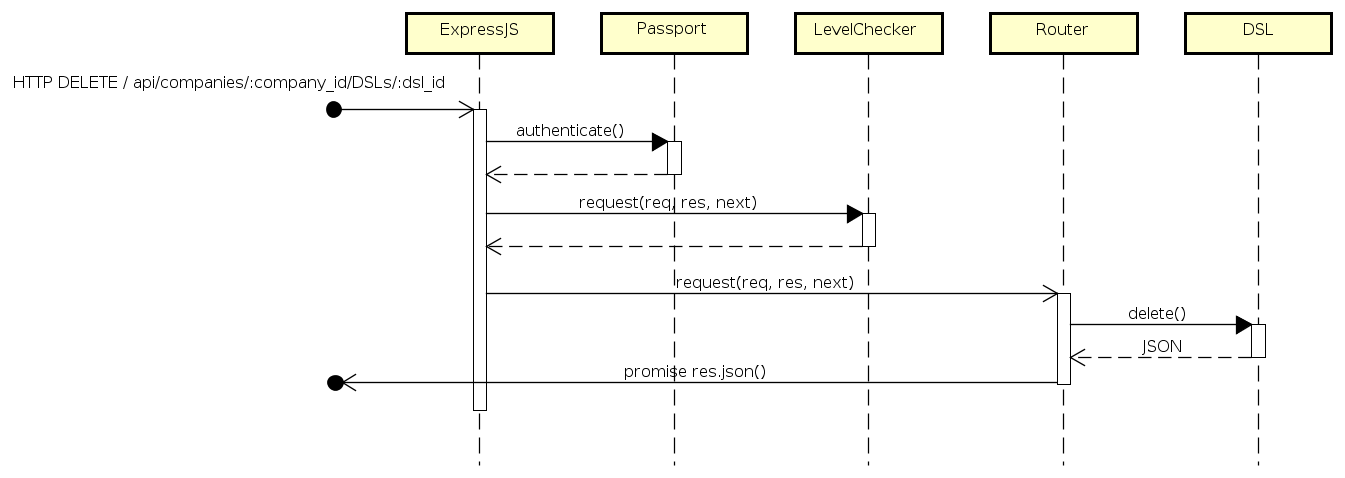
\includegraphics[width=0.8\textwidth]{res/sections/backend/(DELETE)dsl.png}
\caption{Scenario della cancellazione di una specifica DSL}
\end{figure}

\newpage
\subsubsection{Ottenimento della dashboard di un utente}
\textbf{Tipologia:} GET \\
\textbf{API:} /api/:company\_id/Dashboard \\
\textbf{Livello di accesso minimo:} GUEST \\
\textbf{Descrizione:} Ritorna la dashboard di un utente definita da una DSL. \\
\textbf{Scenario:}  
\begin{figure}[h]
\centering
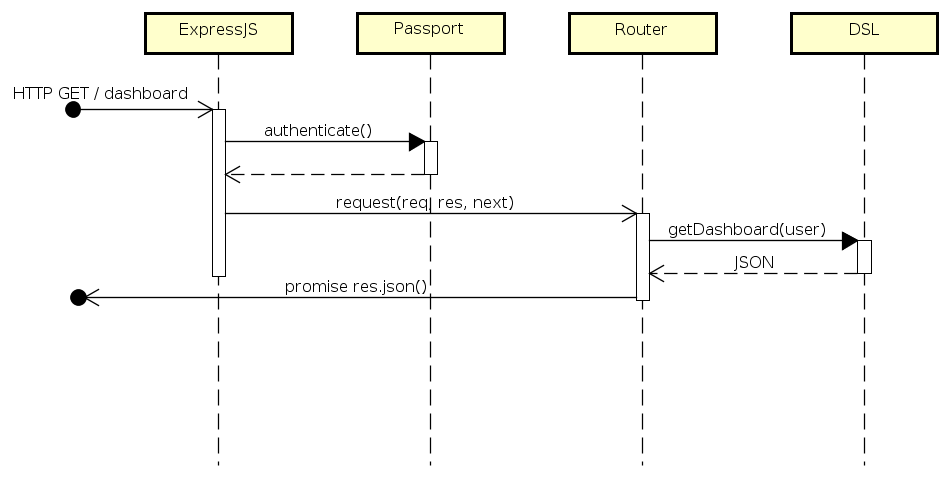
\includegraphics[width=0.8\textwidth]{res/sections/backend/(GET)dashboard.png}
\caption{Scenario dell'ottenimento della dashboard di un utente}
\end{figure}

\newpage
\subsubsection{Esecuzione di una specifica DSL}
\textbf{Tipologia:} GET \\
\textbf{API:} /api/:company\_id/DSL/:dsl\_id/execute \\
\textbf{Livello di accesso minimo:} GUEST \\
\textbf{Descrizione:} Ritorna un JSON contenente i dati richiesti dalla specifica DSL e la struttura su cui inserire i dati. \\
\textbf{Scenario:} 
\begin{figure}[h]
\centering
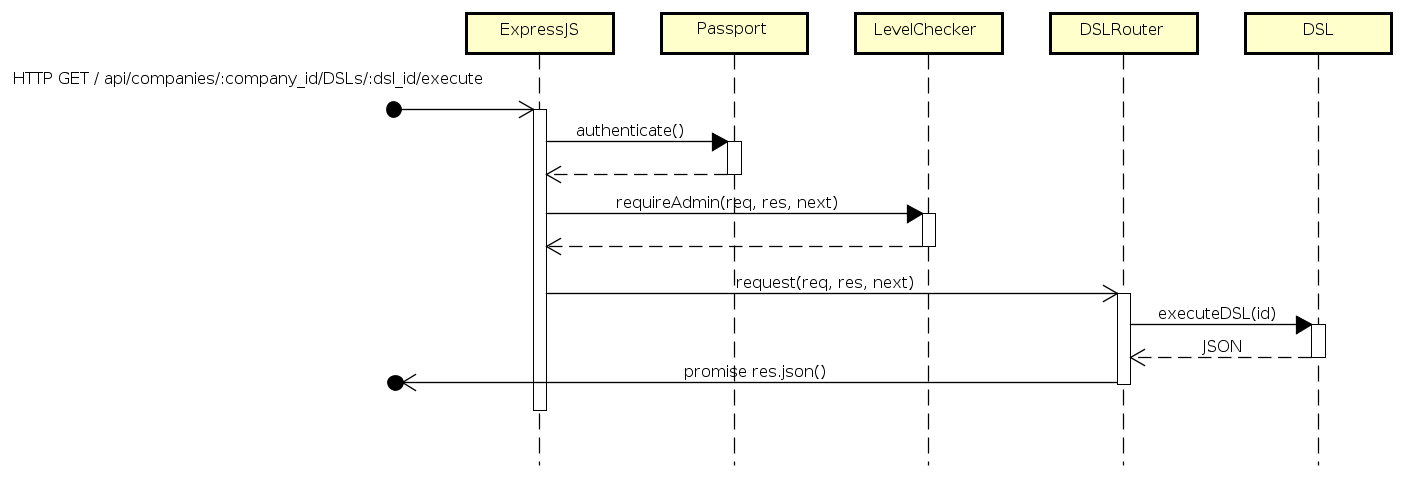
\includegraphics[width=0.8\textwidth]{res/sections/backend/(GET)dslByIDex.png}
\caption{Scenario dell'esecuzione di una specifica DSL}
\end{figure}

\newpage
\subsection{Database}
\textbf{Tipologia:} GET \\
\textbf{API:} /api/:company\_id/database \\
\textbf{Livello di accesso minimo:} MEMBER \\
\textbf{Descrizione:} Ritorna un array contenente i nomi e gli id di ciascun database. \\
\textbf{Scenario:}
\subsubsection{Elenco dei database della company}
\begin{figure}[h]
\centering
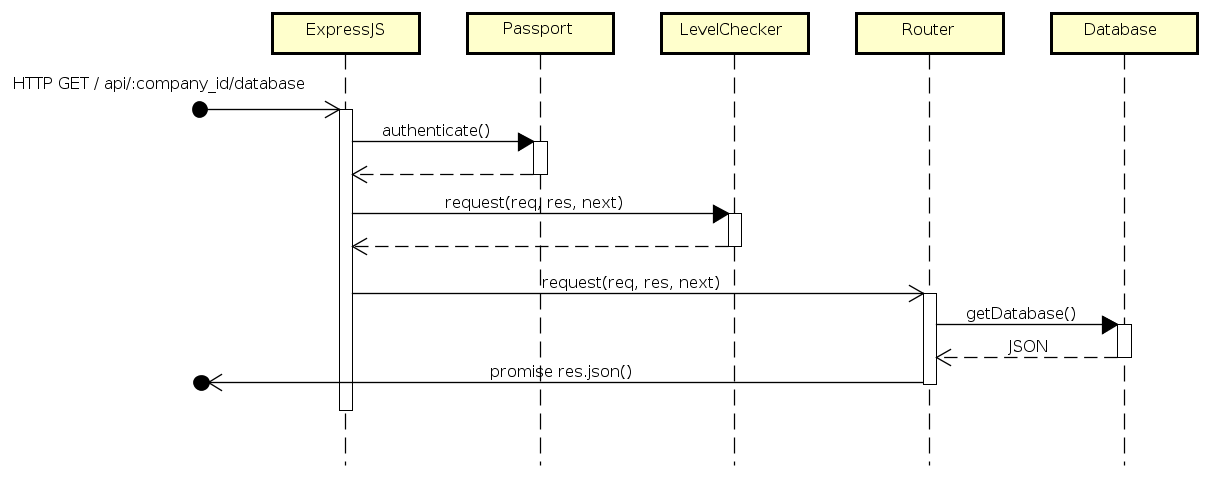
\includegraphics[width=0.8\textwidth]{res/sections/backend/(GET)database.png}
\caption{Scenario dell'elenco dei database propri della company}
\end{figure}

\newpage
\subsubsection{Visualizzazione dati di un database}
\textbf{Tipologia:} GET \\
\textbf{API:} /api/:company\_id/database/:database\_id \\
\textbf{Livello di accesso minimo:} ADMIN \\
\textbf{Descrizione:} Ritorna tutte le informazioni relative al database richiesto. \\
\textbf{Scenario:} 
\begin{figure}[h]
\centering
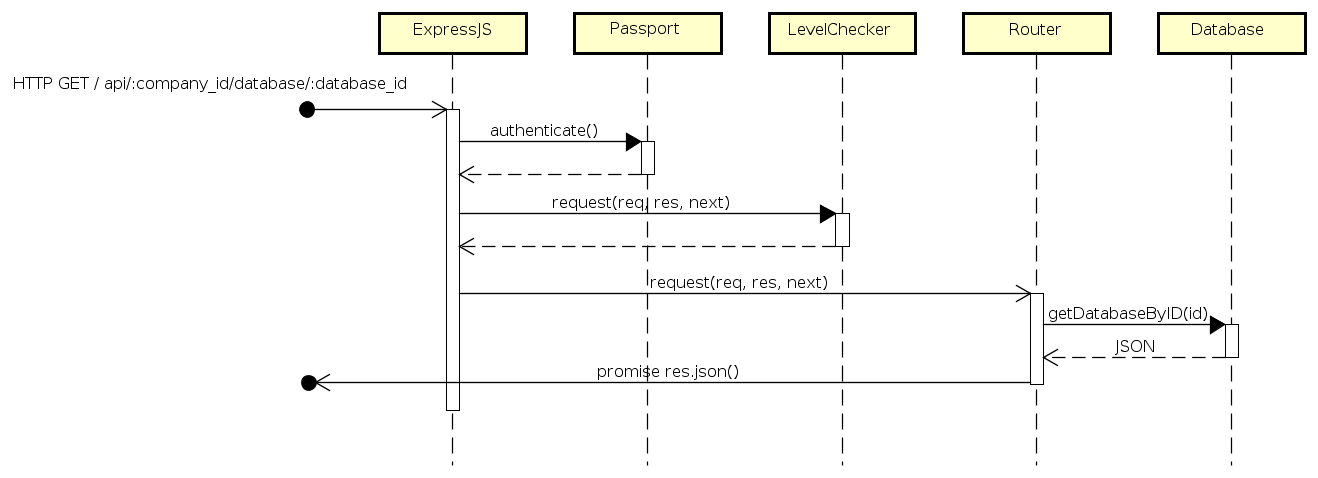
\includegraphics[width=0.8\textwidth]{res/sections/backend/(GET)databaseById.png}
\caption{Scenario della visualizzazione dei dati di un database}
\end{figure}

\newpage
\subsubsection{Aggiunta di un database}
\textbf{Tipologia:} POST \\
\textbf{API:} /api/:company\_id/database \\
\textbf{Livello di accesso minimo:} ADMIN \\
\textbf{Descrizione:} Necessita di una richiesta con body contenete i dati relativi alla connessione del nuovo database. \\
\textbf{Scenario:}
\begin{figure}[h]
\centering
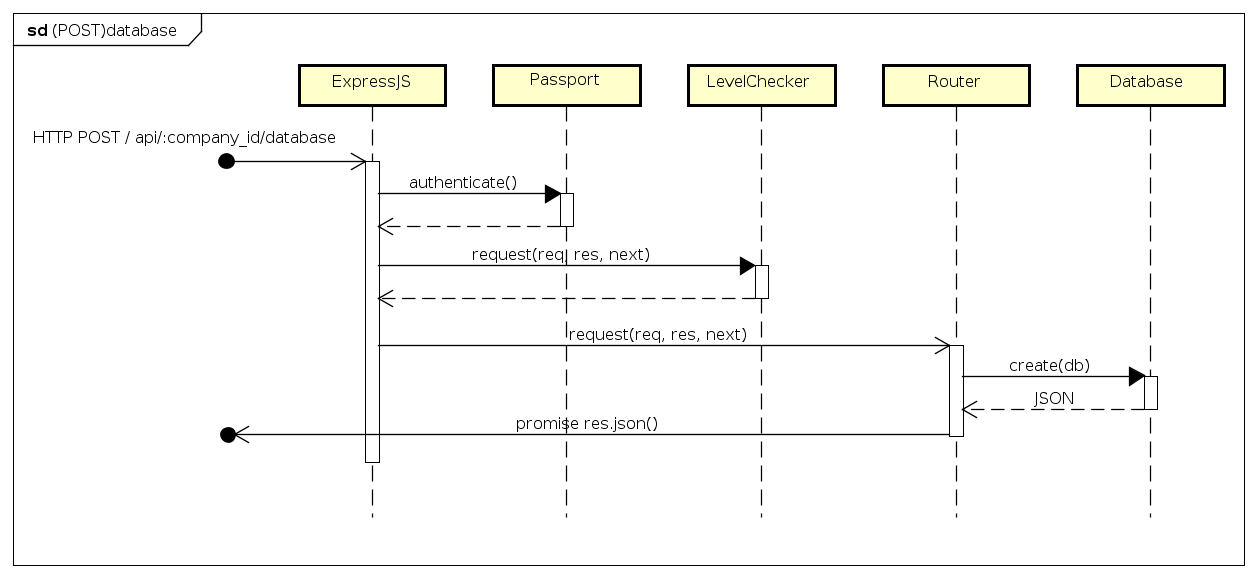
\includegraphics[width=0.8\textwidth]{res/sections/backend/(POST)database.png}
\caption{Scenario della creazione di una specifica DSL}
\end{figure}

\newpage
\subsubsection{Aggiornamento di un database}
\textbf{Tipologia:} PUT \\
\textbf{API:} /api/:company\_id/database/:database\_id \\
\textbf{Livello di accesso minimo:} ADMIN \\
\textbf{Descrizione:} Metodo per aggiornare le informazioni relative alla connessione al database o per aggiornare l'elenco delle collezioni. \\
\textbf{Scenario:}
\begin{figure}[h]
\centering
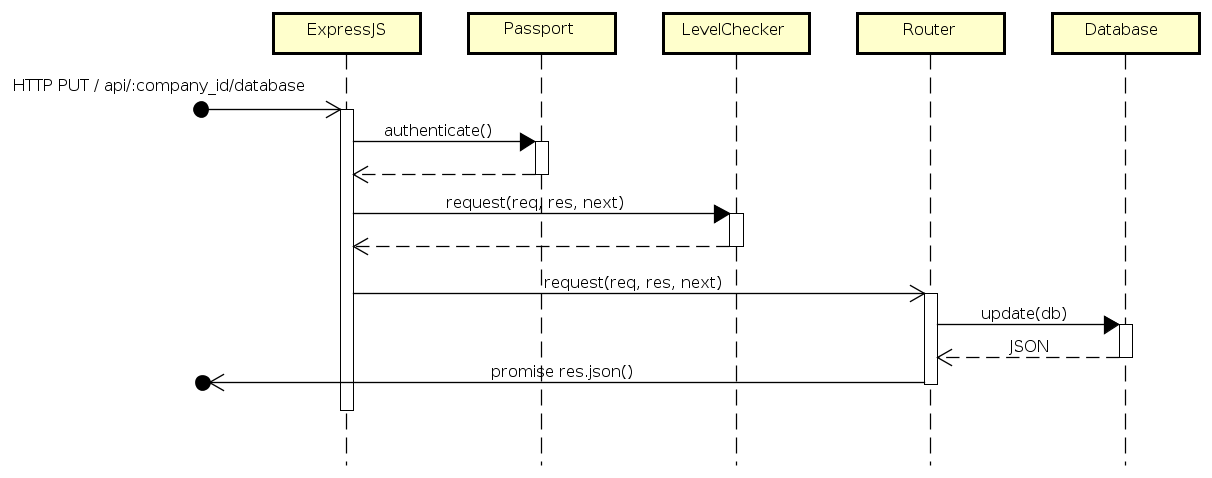
\includegraphics[width=0.8\textwidth]{res/sections/backend/(PUT)database.png}
\caption{Scenario dell'aggiornamento di un database}
\end{figure}

\newpage
\subsubsection{Cancellazione di un database}
\textbf{Tipologia:} DELETE \\
\textbf{API:} /api/:company\_id/database/:database\_id \\
\textbf{Livello di accesso minimo:} ADMIN \\
\textbf{Descrizione:} Elimina il database selezionato e tutte le DSL che lo utilizzano. \\
\textbf{Scenario:} 
\begin{figure}[h]
\centering
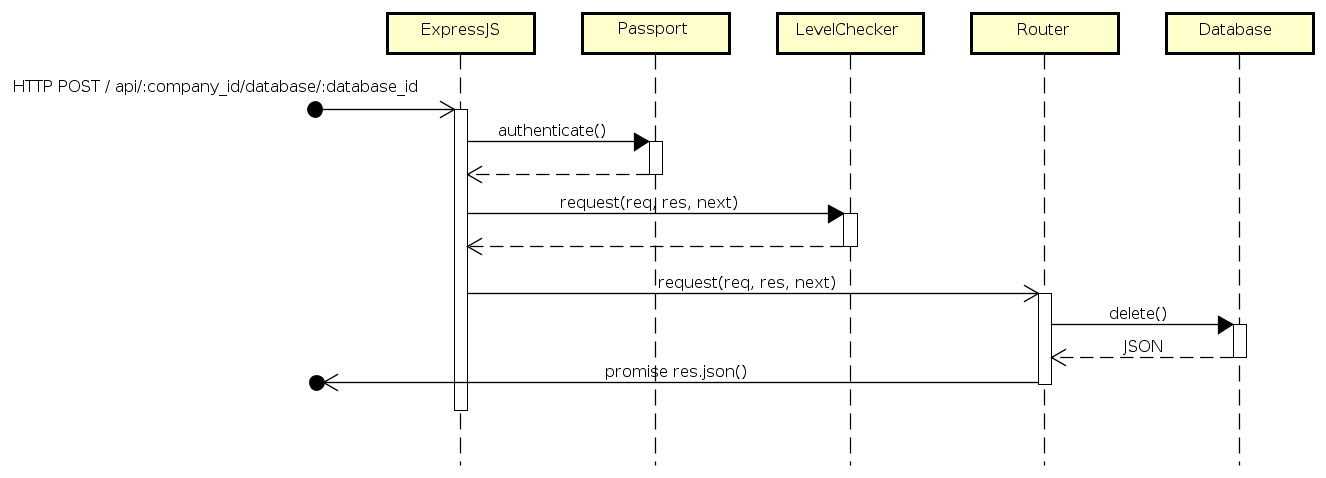
\includegraphics[width=0.8\textwidth]{res/sections/backend/(DELETE)database.png}
\caption{Scenario della cancellazione di un database}
\end{figure}

\newpage
\subsubsection{Visualizzazione collections di un database}
\textbf{Tipologia:} GET \\
\textbf{API:} /api/:company\_id/database/:database\_id/collection \\
\textbf{Livello di accesso minimo:} MEMBER \\
\textbf{Descrizione:} Ritorna un array di collection relative ad un database a cui l'utente ha accesso. \\
\textbf{Scenario:} 
\begin{figure}[h]
\centering
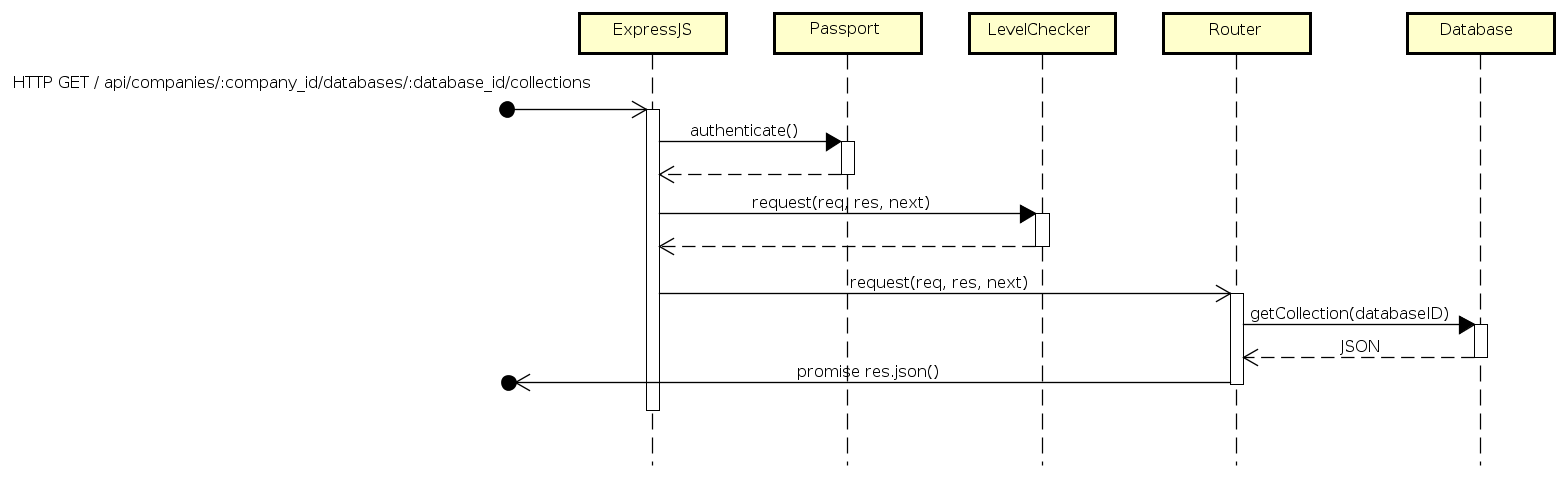
\includegraphics[width=0.8\textwidth]{res/sections/backend/(GET)collection.png}
\caption{Scenario della visualizzazione collections di un database}
\end{figure}

\newpage
\subsection{Super admin}
\subsubsection{Ottenimento informazioni delle companies}
\textbf{Tipologia:} GET \\
\textbf{API:} /api/admin/company \\
\textbf{Descrizione:} Restituisce un array di JSON contenenti le informazioni relative alle company presenti nell'applicazione. \\
\textbf{Scenario:} 
\begin{figure}[h]
\centering
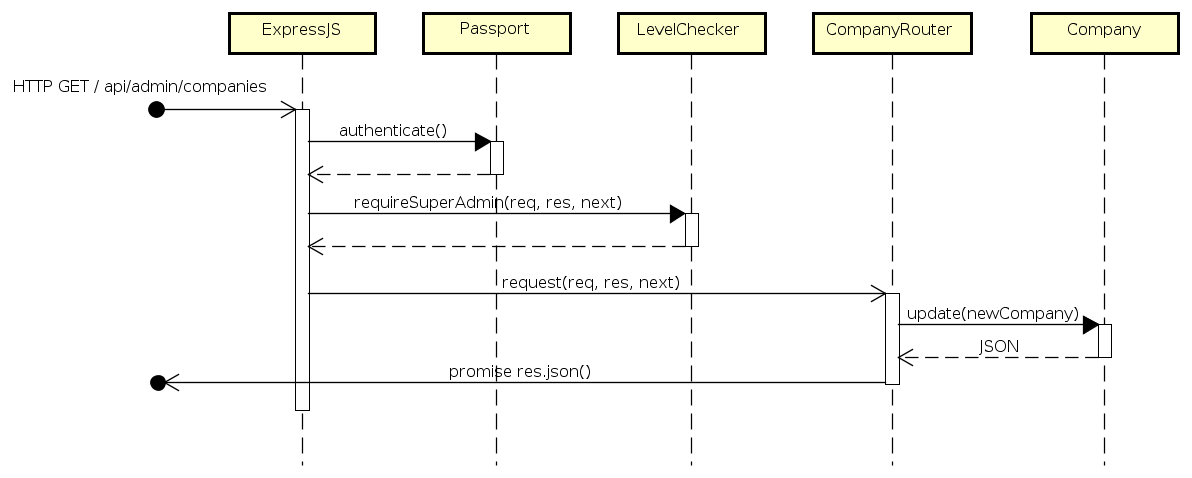
\includegraphics[width=0.8\textwidth]{res/sections/backend/(GET)companySA.png}
\caption{Scenario dell'ottenimento informazioni delle companies}
\end{figure}

\newpage
\subsubsection{Aggiunta di un super admin}
\textbf{Tipologia:} POST \\
\textbf{API:} /api/admin/superadmin \\
\textbf{Descrizione:} Necessita di una richiesta con body contenente le informazioni relative al superadmin da creare. \\
\textbf{Scenario:} 
\begin{figure}[h]
\centering
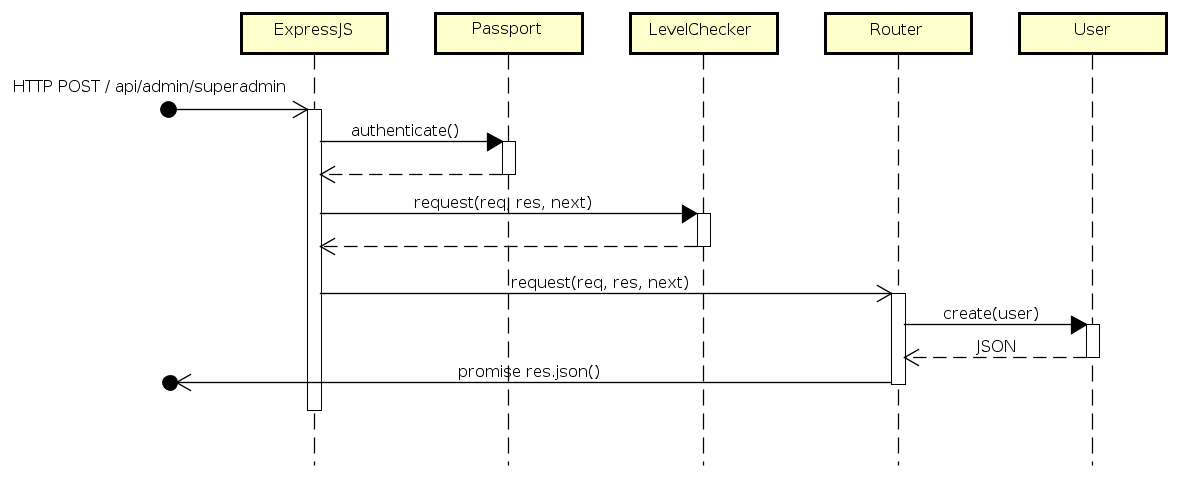
\includegraphics[width=0.8\textwidth]{res/sections/backend/(POST)superadmin.png}
\caption{Scenario dell'aggiunta di un super admin}
\end{figure}

\newpage
\subsubsection{Aggiunta di un utente}
\textbf{Tipologia:} POST \\
\textbf{API:} /api/admin/company/:company\_id/user \\
\textbf{Descrizione:} Necessita di una richiesta con body contenente le informazioni relative all'utente da creare per la company individuata da company\_id. \\
\textbf{Scenario:} 
\begin{figure}[h]
\centering
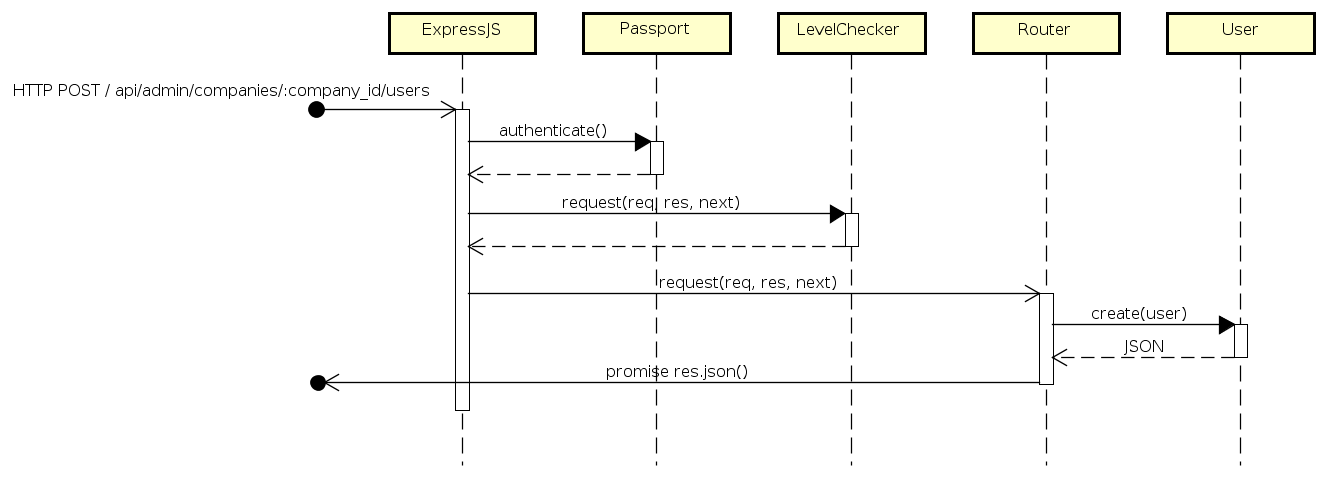
\includegraphics[width=0.8\textwidth]{res/sections/backend/(POST)userSA.png}
\caption{Scenario dell'aggiunta di un utente}
\end{figure}